% ------------------------------------------------------------------------------
% TYPO3 CMS 8.3 - What's New (English Version)
%
% @author	Patrick Lobacher <patrick@lobacher.de> and Michael Schams <schams.net>
% @license	Creative Commons BY-NC-SA 3.0
% @link		http://typo3.org/download/release-notes/whats-new/
% @language	English
% ------------------------------------------------------------------------------
% LTXE-CHAPTER-UID:		07b25346-95b1df21-a6ebe09a-49f53f41
% LTXE-CHAPTER-NAME:	Backend User Interface
% ------------------------------------------------------------------------------

\section{Interfaz de Usuario de Backend}
\begin{frame}[fragile]
	\frametitle{Interfaz de Usuario de Backend}

	\begin{center}\huge{Capítulo 1:}\end{center}
	\begin{center}\huge{\color{typo3darkgrey}\textbf{Interfaz de Usuario de Backend}}\end{center}

\end{frame}

% ------------------------------------------------------------------------------
% LTXE-SLIDE-START
% LTXE-SLIDE-UID:		1b8c2339-be35ad00-9ad2dfc8-6cc24417
% LTXE-SLIDE-ORIGIN:	a5b4032f-741b8eea-643674fb-4dc14f50 English
% LTXE-SLIDE-TITLE:		!Feature: #20446 - Clear cache entry in context menu
% LTXE-SLIDE-REFERENCE:	!Feature-20446-ClearCacheEntryInContextMenu.rst
% ------------------------------------------------------------------------------
\begin{frame}[fragile]
	\frametitle{Interfaz de Usuario de Backend}
	\framesubtitle{Entrada "Vaciar Caché" en Menú de Contexto}

	Una nueva entrada ha sido añadida al menú de contexto del árbol de páginas. El ítem es localizado dentro de las "Acciones de Página"
	y permite vaciar la caché de la página seleccionada.

	\begin{figure}
		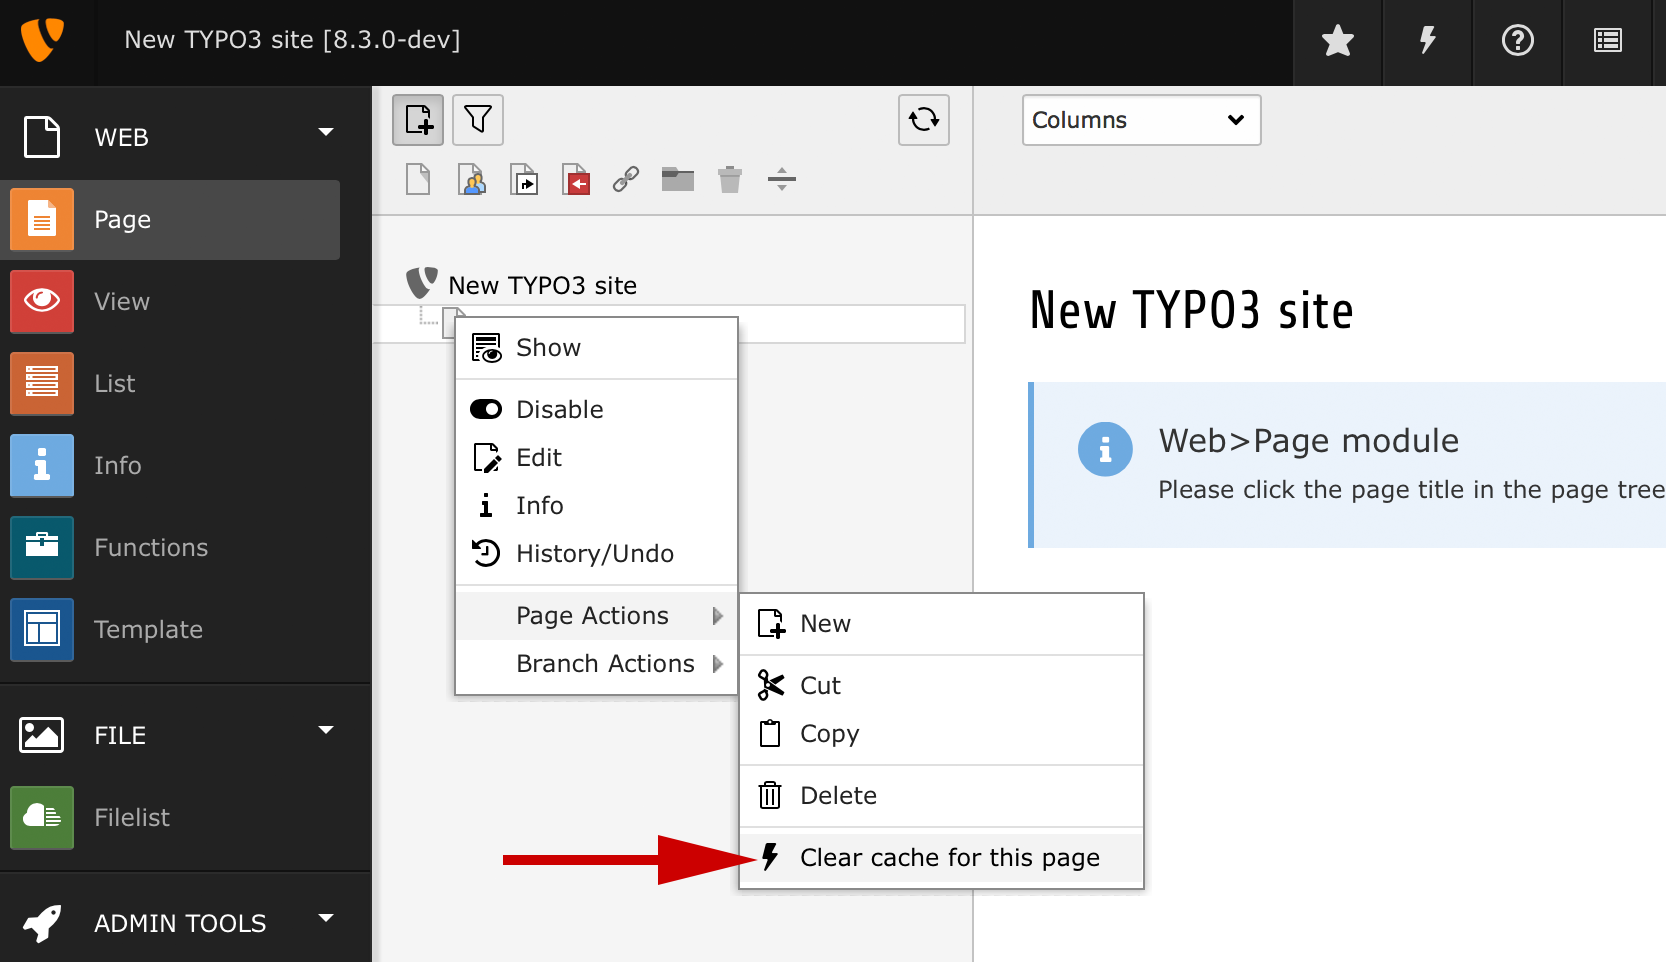
\includegraphics[width=0.70\linewidth]{BackendUserInterface/20446.png}
	\end{figure}

\end{frame}

% ------------------------------------------------------------------------------
% LTXE-SLIDE-START
% LTXE-SLIDE-UID:		66e012f1-9418a2f9-c68b2381-9ccbba1c
% LTXE-SLIDE-ORIGIN:	5b0090eb-13043388-8c4dee34-6cac1521 English
% LTXE-SLIDE-TITLE:		!Feature: #76072 - Ogg, flac and opus support
% LTXE-SLIDE-REFERENCE:	!Feature-76072-OggFlacAndOpusSupport.rst
% ------------------------------------------------------------------------------
\begin{frame}[fragile]
	\frametitle{Interfaz de Usuario de Backend}
	\framesubtitle{Soporte Ogg, Flac y Opus}

	Se ha añadido soporte para los siguientes formatos abiertos en el campo media:
	\texttt{ogg}, \texttt{flac} and \texttt{opus}

	\begin{figure}
		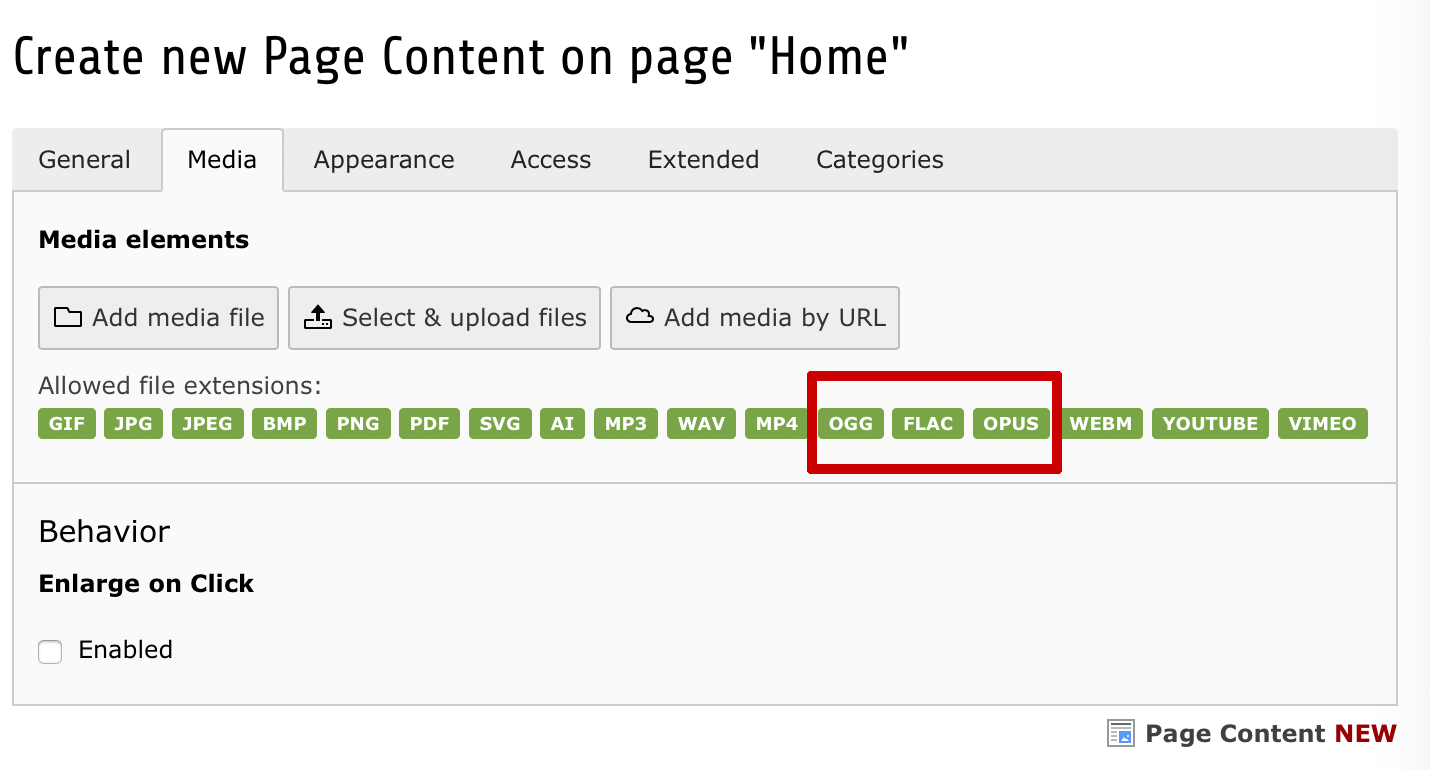
\includegraphics[width=0.70\linewidth]{BackendUserInterface/76072.png}
	\end{figure}

\end{frame}


